\documentclass[../DoAn.tex]{subfiles}
\begin{document}


Chương 2 tập trung vào việc nghiên cứu hiện trạng, phân tích các yêu cầu nghiệp vụ và đặc tả kiến trúc chức năng chi tiết của sàn thương mại điện tử đa nhà bán hàng. Để xây dựng một nền tảng phần mềm hoạt động ổn định và đáp ứng tốt các yêu cầu chịu tải cao, nội dung chương sẽ lần lượt trình bày về: khảo sát các hệ thống thương mại điện tử hiện tại và đề xuất danh sách chức năng ưu tiên trong phần \ref{section:2.1}; phác thảo tổng quan hệ thống thông qua các biểu đồ ca sử dụng (Use Case) tổng quát và phân rã các nhóm nghiệp vụ chính trong phần \ref{section:2.2}; đặc tả chi tiết luồng hoạt động của các ca sử dụng then chốt trong phần \ref{section:2.3}; và sau cùng là thiết lập hệ thống các yêu cầu phi chức năng về hiệu năng, bảo mật và khả năng mở rộng của sản phẩm trong phần \ref{section:2.4}.

\section{Khảo sát hiện trạng}
\label{section:2.1}
Khảo sát chi tiết hiện trạng kỹ thuật và nghiệp vụ được tổng hợp từ ba nguồn chính nhằm định vị rõ ràng các vấn đề cốt lõi cần giải quyết:
(i) *Từ phía người dùng và thương nhân:* Người mua mong muốn một hệ thống thanh toán mượt mà, minh bạch về giá, áp dụng được nhiều lớp mã giảm giá cùng lúc và giao tiếp tức thời với người bán. Thương nhân cần bảng số liệu trực quan, cập nhật nhanh để quản trị dòng tiền, hàng tồn kho và các chương trình khuyến mãi riêng biệt.
(ii) *Từ các hệ thống sẵn có (Shopify, Woocommerce):* Các nền tảng này hỗ trợ tốt mô hình một cửa hàng (Single-shop) nhưng gặp nhiều khó khăn hoặc yêu cầu kiến trúc plugin cồng kềnh để vận hành mô hình đa nhà bán hàng (Multi-vendor) – nơi đơn hàng cần được tách tự động theo nhà bán, giá vận chuyển tính riêng biệt và voucher áp dụng theo cấp độ cửa hàng.
(iii) *Đánh giá hiệu năng dưới tải cao:* Các hệ thống cũ thường thiết kế cơ sở dữ liệu dạng khóa quan hệ truyền thống, áp dụng kỹ thuật đọc-ghi gián tiếp (Read-Modify-Write) dẫn đến thời gian phản hồi chậm khi nhiều người cùng đặt hàng, gây ra lỗi nghiêm trọng về bán quá mức tồn kho thực tế (overselling) và sập hệ thống xác thực khi bị tấn công spam OTP.

Bảng \ref{table:survey} dưới đây trình bày so sánh chi tiết ưu nhược điểm của các giải pháp hiện tại so với kiến trúc đề xuất của đồ án.

\begin{longtable}{|p{2.5cm}|p{6cm}|p{6cm}|}
\hline
\textbf{Tiêu chí} & \textbf{Các hệ thống truyền thống} & \textbf{Hệ thống đề xuất trong đồ án} \\ \hline
\end{longtable}
\begin{longtable}{|p{2.5cm}|p{6.1cm}|p{6.1cm}|}
\hline
\textbf{Mô hình} & Hỗ trợ tốt Single-shop; cấu hình Multi-vendor phức tạp. & Thiết kế chuyên biệt cho Multi-vendor, tự động tách đơn hàng theo shop. \\ \hline
\textbf{Xử lý kho} & Dễ bị lỗi bán quá mức (Oversell) dưới tải cao do thiếu cơ chế atomic. & Triệt tiêu lỗi Oversell nhờ cơ chế giữ kho nguyên tử (Atomic DB Reservation). \\ \hline
\textbf{Mã giảm giá} & Áp dụng voucher một lớp đơn giản cho toàn giỏ hàng. & Động cơ tính giảm giá bảo mật 4 lớp xử lý hoàn toàn tại phía backend. \\ \hline
\textbf{Bảo mật} & Xác thực session/token thông thường; dễ bị Brute-force/leak token qua URL. & Bảo mật xác thực đa lớp bảo vệ bởi Redis rate-limit và cơ chế Refresh Token Rotation. \\ \hline
\textbf{Cá nhân hóa} & Hiển thị sản phẩm theo phân loại tĩnh thông thường. & Tích hợp bộ khuyến nghị lai Hybrid (Collaborative + Content-based) có Time Decay. \\ \hline
\end{longtable}
\label{table:survey}

Từ các phân tích trên, đồ án xác định các tính năng phần mềm quan trọng nhất cần tập trung phát triển bao gồm: Đăng nhập/Đăng ký hợp nhất an toàn, Giỏ hàng thông minh phân tách đơn theo nhà bán, Động cơ tính toán giảm giá đa lớp bảo mật, Thanh toán trực tuyến tích hợp và Hệ thống phân tích số liệu động Recharts dành cho Merchant.

\section{Tổng quan chức năng}
\label{section:2.2}
Hệ thống sàn thương mại điện tử đa nhà bán hàng được phân tích và thiết kế hướng đối tượng với ba tác nhân (Actors) chính tham gia tương tác:
\begin{itemize}
\item \textbf{Khách hàng (Buyer):} Người mua hàng trên hệ thống, có quyền tìm kiếm sản phẩm, xem danh sách gợi ý cá nhân hóa, quản lý giỏ hàng, áp dụng các mã giảm giá hợp lệ, đặt hàng qua COD hoặc Stripe/VNPay, theo dõi đơn hàng, viết đánh giá và chat trực tiếp với từng nhà bán hàng.
\item \textbf{Đối tác bán hàng (Vendor/Seller):} Người đăng ký gian hàng từ tài khoản người dùng của mình. Có quyền đăng sản phẩm và biến thể (kèm giá, kích thước, màu sắc), quản lý tồn kho, cấu hình mã giảm giá (Shop Voucher) riêng của cửa hàng, cập nhật trạng thái đơn hàng, giao tiếp với khách hàng và theo dõi biểu đồ thống kê doanh thu Recharts.
\item \textbf{Quản trị viên (Platform Admin):} Quản lý toàn bộ hệ thống ở mức cao nhất, có quyền kiểm duyệt nhà bán hàng, quản lý danh mục sản phẩm nền, cấu hình mã giảm giá toàn sàn (Platform Voucher / Shipping Discount) và giám sát chỉ số tăng trưởng chung của toàn sàn.
\end{itemize}

\subsection{Biểu đồ use case tổng quát}
\label{subsection:2.2.1}
Biểu đồ ca sử dụng tổng quát của hệ thống phác thảo các tương tác cơ bản giữa ba tác nhân chính và các nhóm chức năng lớn bao gồm: Quản lý tài khoản và bảo mật, Nghiệp vụ mua bán hàng hóa, Quản trị gian hàng \& Phân tích số liệu, và Hệ thống tương tác thời gian thực (Chat/Notification) như mô tả trong Hình \ref{fig:general_use_case}.

\begin{figure}[htbp]
    \centering
    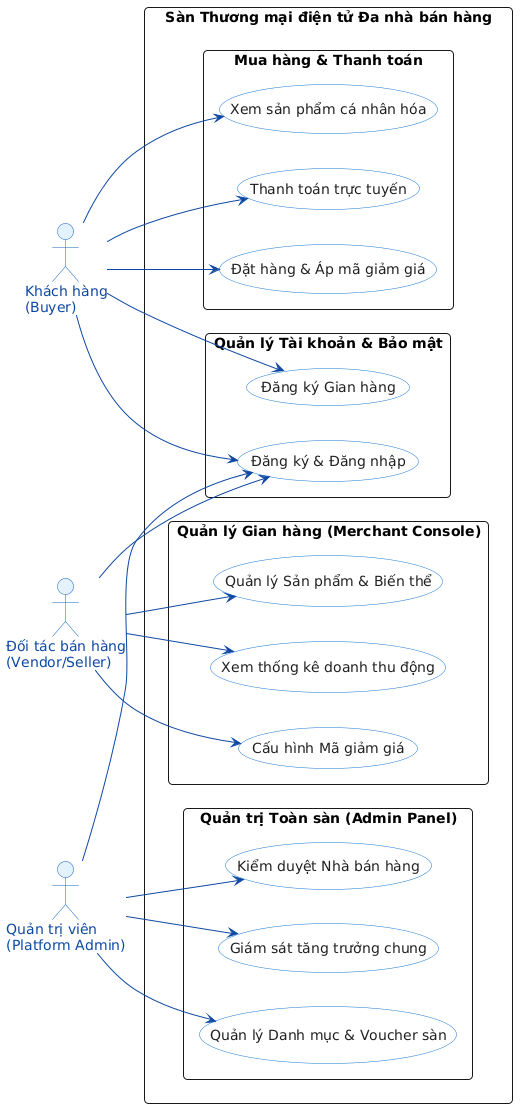
\includegraphics[width=0.85\textwidth]{images/general_use_case.png}
    \caption{Biểu đồ ca sử dụng (Use Case) tổng quát của hệ thống}
    \label{fig:general_use_case}
\end{figure}

\subsection{Biểu đồ use case phân rã các phân hệ nghiệp vụ chính}
\label{subsection:2.2.2}
Để làm rõ cấu trúc chức năng, các nhóm ca sử dụng lớn được phân rã thành các ca sử dụng thành phần:

\subsubsection{Phân hệ Quản lý tài khoản và Bảo mật (Auth \& Security)}
Tác nhân Khách hàng và Đối tác bán hàng tương tác với phân hệ bảo mật thông qua các ca sử dụng phân rã bao gồm:
\begin{itemize}
    \item \textbf{Đăng ký tài khoản:} Nhập thông tin và bắt buộc xác minh mã OTP 6 số qua email.
    \item \textbf{Đăng nhập hệ thống:} Hỗ trợ mật mã thông thường (bảo vệ bởi IP/Email Rate limit) hoặc Đăng nhập nhanh qua Google OAuth.
    \item \textbf{Đăng ký gian hàng (Vendor Register):} Cho phép tài khoản người mua nâng cấp lên tài khoản nhà bán hàng bằng cách bổ sung tên shop, địa chỉ và số điện thoại mà không phải tạo tài khoản mới.
    \item \textbf{Khôi phục mật khẩu:} Gửi mã token đặt lại mật khẩu bảo mật qua email người dùng.
\end{itemize}

Chi tiết các mối tương tác và sự liên kết giữa các ca sử dụng trong phân hệ Tài khoản và Bảo mật được thể hiện rõ nét trong Hình \ref{fig:auth_security_use_case}.

\begin{figure}[htbp]
    \centering
    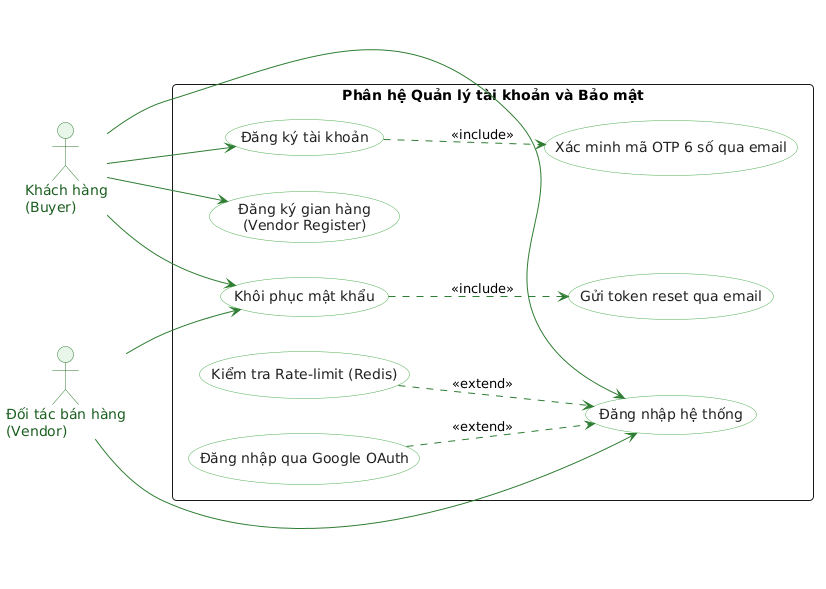
\includegraphics[width=0.85\textwidth]{images/auth_security_use_case.png}
    \caption{Biểu đồ ca sử dụng phân rã phân hệ Quản lý tài khoản và Bảo mật}
    \label{fig:auth_security_use_case}
\end{figure}

\subsubsection{Phân hệ Mua hàng và Thanh toán (Ordering \& Payment)}
Người mua tương tác trực tiếp với các ca sử dụng cốt lõi:
\begin{itemize}
    \item \textbf{Xem sản phẩm cá nhân hóa:} Hệ thống tự động tính toán điểm Interaction Score để đưa ra danh sách sản phẩm gợi ý phù hợp nhất.
    \item \textbf{Áp dụng Voucher 4 lớp:} Người dùng chọn mã giảm giá. Hệ thống backend tự động phân loại, kiểm tra điều kiện áp dụng và trừ tiền theo đúng thứ tự ưu tiên.
    \item \textbf{Giữ kho nguyên tử:} Khi xác nhận đặt hàng, hệ thống khóa tài nguyên kho của tổng sản phẩm và biến thể ngay dưới DB để tránh oversell.
    \item \textbf{Thanh toán trực tuyến:} Gọi API tạo checkout session qua Stripe/VNPay, xử lý phản hồi đồng bộ qua Webhook.
\end{itemize}

Sơ đồ phân rã ca sử dụng của phân hệ Mua hàng và Thanh toán được biểu diễn trong Hình \ref{fig:ordering_payment_use_case}.

\begin{figure}[htbp]
    \centering
    
\includegraphics[width=0.85\textwidth]{images/ordering_payment_use_case.png}
    \caption{Biểu đồ ca sử dụng phân rã phân hệ Mua hàng và Thanh toán}
    \label{fig:ordering_payment_use_case}
\end{figure}

\subsubsection{Phân hệ Quản lý gian hàng (Merchant Console)}
Thương nhân quản trị các hoạt động thương mại thông qua bảng điều khiển độc lập:
\begin{itemize}
    \item \textbf{Quản lý sản phẩm và biến thể:} Đăng tải, chỉnh sửa thông tin, đặt khóa biến thể (`variantKey`) cấu hình tồn kho chi tiết.
    \item \textbf{Cấu hình mã giảm giá riêng (Shop Voucher):} Thiết lập mã giảm giá theo phần trăm hoặc số tiền cố định áp dụng riêng cho subtotal của shop.
    \item \textbf{Xem thống kê doanh thu động (Stats):} Biểu đồ Recharts phân tích dòng doanh thu theo ngày, số lượng đơn theo tháng và cảnh báo sản phẩm sắp hết hàng (tồn kho $\le 5$).
\end{itemize}

Các chức năng chi tiết thuộc phân hệ Quản lý gian hàng dành cho đối tác bán hàng được thể hiện trong Hình \ref{fig:merchant_console_use_case}.

\begin{figure}[htbp]
    \centering
    
\includegraphics[width=0.85\textwidth]{images/merchant_console_use_case.png}
    \caption{Biểu đồ ca sử dụng phân rã phân hệ Quản lý gian hàng}
    \label{fig:merchant_console_use_case}
\end{figure}

\subsection{Quy trình nghiệp vụ Đặt hàng giữ kho và Thanh toán đồng thời}
\label{subsection:2.2.3}
Hệ thống thiết kế quy trình nghiệp vụ đặt hàng và thanh toán đồng thời cực kỳ chặt chẽ nhằm bảo toàn tồn kho vật lý và tránh lỗi thanh toán trùng lặp. Luồng hoạt động tổng thể tích hợp nhiều ca sử dụng diễn ra như sau:

\begin{enumerate}
    \item \textbf{Bước 1:} Khách hàng thêm các sản phẩm với biến thể cụ thể vào giỏ hàng và tiến hành checkout.
    \item \textbf{Bước 2:} Hệ thống gửi danh sách sản phẩm và các mã voucher lên endpoint \texttt{/api/order/preview}. Backend thực hiện tính toán thử bảng kê tiền tệ 4 lớp và trả về bảng tính chi tiết.
    \item \textbf{Bước 3:} Người dùng xác nhận chọn thanh toán trực tuyến (Stripe hoặc VNPay) kèm \texttt{idempotencyKey} sinh từ client.
    \item \textbf{Bước 4:} Backend gọi hàm \texttt{reserveStockByUnits} tiến hành kiểm tra tồn kho nguyên tử.
    \begin{itemize}
        \item \textit{Nếu đủ hàng:} Tồn kho tổng và tồn kho biến thể lập tức bị trừ, đơn hàng được tạo với trạng thái \texttt{PENDING\_PAYMENT} (Chờ thanh toán) kèm thời gian giữ kho \texttt{reservationExpiresAt} mặc định là 15 phút.
        \item \textit{Nếu thiếu hàng ở bất kỳ sản phẩm nào:} Trả về mã lỗi \texttt{OUT\_OF\_STOCK} kèm số lượng khả dụng thực tế để giao diện thông báo, toàn bộ quá trình bị hủy bỏ.
    \end{itemize}
    \item \textbf{Bước 5:} Tạo checkout session với Stripe/VNPay trỏ đến trang thanh toán an toàn của cổng thanh toán.
    \item \textbf{Bước 6:} Khách hàng thực hiện thanh toán trên giao diện cổng thanh toán.
    \begin{itemize}
        \item \textit{Trường hợp thành công:} Cổng thanh toán gửi tín hiệu Webhook về Backend. Backend kiểm tra tính hợp lệ, đổi trạng thái đơn sang \texttt{CONFIRMED} (Đã xác nhận), hoàn tất tăng biến đếm số lượng bán (\texttt{sold}), xóa các sản phẩm khỏi giỏ hàng của user và gửi thông báo đẩy realtime qua Socket.IO tới các Vendor liên quan.
        \item \textit{Trường hợp thất bại hoặc quá hạn 15 phút không thanh toán:} Job quét tự động của server (Cron Sweeper) phát hiện đơn \texttt{PENDING\_PAYMENT} hết hạn, chuyển trạng thái đơn sang \texttt{EXPIRED} (Quá hạn) và gọi hàm \texttt{releaseStockByUnits} cộng trả lại số lượng tồn kho nguyên tử cho sản phẩm và biến thể, đồng thời hoàn lại lượt sử dụng cho các voucher liên quan.
    \end{itemize}
\end{enumerate}

\begin{figure}[htbp]
    \centering
    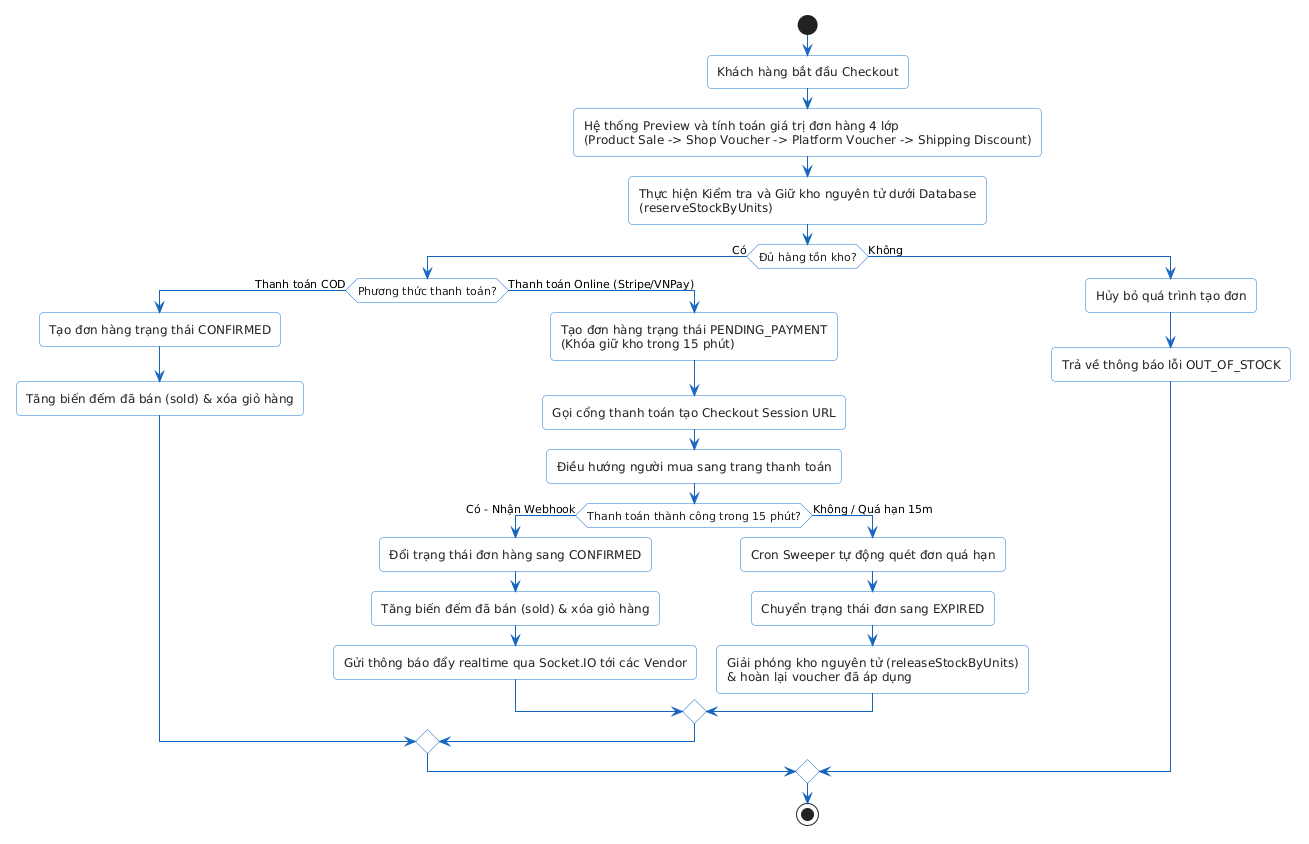
\includegraphics[width=0.80\textwidth]{images/checkout_process.png}
    \caption{Biểu đồ hoạt động quy trình nghiệp vụ Đặt hàng - Giữ kho - Thanh toán đồng thời}
    \label{fig:checkout_process}
\end{figure}

Để làm rõ thứ tự tương tác, lời gọi API và luồng dữ liệu thời gian thực giữa Khách hàng, Client, Backend Server, Cơ sở dữ liệu và Cổng thanh toán ngoại vi, Hình \ref{fig:order_payment_sequence} dưới đây mô tả chi tiết biểu đồ tuần tự (Sequence Diagram) của quy trình nghiệp vụ phức tạp này.

\begin{figure}[htbp]
    \centering
    
\includegraphics[width=0.98\textwidth]{images/order_payment_sequence.png}
    \caption{Biểu đồ tuần tự chi tiết quy trình nghiệp vụ Đặt hàng, Giữ kho nguyên tử và Thanh toán đồng thời}
    \label{fig:order_payment_sequence}
\end{figure}

\section{Đặc tả chức năng}
\label{section:2.3}
Dưới đây là đặc tả chi tiết của 4 ca sử dụng (Use Case) cốt lõi đóng vai trò quan trọng nhất trong việc vận hành toàn hệ thống.

\subsection{Đặc tả ca sử dụng 1: Đăng nhập hệ thống hợp nhất và Bảo mật}
\begin{itemize}
    \item \textbf{Tên ca sử dụng:} Đăng nhập hệ thống (Login).
    \item \textbf{Tác nhân chính:} Khách hàng, Đối tác bán hàng.
    \item \textbf{Tiền điều kiện:} Người dùng đã đăng ký tài khoản và xác minh email thành công.
    \item \textbf{Hậu điều kiện:} Người dùng đăng nhập thành công, nhận được \texttt{accessToken} lưu trong cookie bảo mật HttpOnly và giao diện điều hướng theo đúng quyền hạn (\texttt{role: user} hoặc \texttt{role: vendor}).
    \item \textbf{Luồng sự kiện chính:}
    \begin{enumerate}
        \item Người dùng truy cập trang đăng nhập, điền email và mật khẩu hoặc chọn Đăng nhập qua Google.
        \item Hệ thống kiểm tra tần suất yêu cầu trong Redis rate-limiter. Nếu vượt ngưỡng cho phép, trả về lỗi HTTP 429 và hiển thị thời gian chờ.
        \item Hệ thống kiểm tra thông tin tài khoản dưới DB. Nếu khớp mật khẩu (sau khi giải mã qua \texttt{bcrypt}), hệ thống cấp cặp token Access và Refresh Token.
        \item Hệ thống ghi Access và Refresh Token vào Cookie bảo mật với cờ \texttt{httpOnly} và \texttt{sameSite: lax}.
        \item Giao diện nhận được phản hồi thành công, lấy thông tin profile và mở quyền truy cập tương ứng.
    \end{enumerate}
    \item \textbf{Luồng sự kiện phát sinh (Ngoại lệ):}
    \begin{itemize}
        \item \textit{Tại bước 3 (Thông tin sai):} Hệ thống trả về lỗi chung ``Invalid credentials'' mà không chỉ rõ email hay password sai để tránh dò tìm tài khoản.
        \item \textit{Tại bước 3 (Email chưa xác minh):} Trả về lỗi ``Email chưa được xác minh'', hệ thống tự tạo mã OTP mới gửi về email và chuyển hướng người dùng sang trang nhập mã OTP xác thực.
    \end{itemize}
\end{itemize}

\subsection{Đặc tả ca sử dụng 2: Đặt hàng và Giữ kho nguyên tử (Place Order)}
\begin{itemize}
    \item \textbf{Tên ca sử dụng:} Đặt hàng và Giữ kho nguyên tử (Place Order).
    \item \textbf{Tác nhân chính:} Khách hàng.
    \item \textbf{Tiền điều kiện:} Khách hàng đã đăng nhập hệ thống và có ít nhất một sản phẩm hợp lệ trong giỏ hàng.
    \item \textbf{Hậu điều kiện:} Đơn hàng được tạo lập thành công trong cơ sở dữ liệu với trạng thái thích hợp, số lượng kho của các sản phẩm liên quan được cập nhật chính xác và an toàn.
    \item \textbf{Luồng sự kiện chính:}
    \begin{enumerate}
        \item Khách hàng nhấn nút ``Đặt hàng'' trên giao diện thanh toán. Client gửi request kèm giỏ hàng, địa chỉ giao hàng, danh sách mã voucher và \texttt{idempotencyKey}.
        \item Backend kiểm tra trùng lặp thông qua \texttt{idempotencyKey} và \texttt{userId}. Nếu đơn hàng đã tồn tại, trả ngay kết quả cũ để tránh tạo đơn lặp.
        \item Hệ thống gọi hàm \texttt{reserveStockByUnits} để kiểm tra và giảm trừ tổng kho cùng kho biến thể trực tiếp dưới DB bằng câu lệnh cập nhật nguyên tử.
        \item Hệ thống tải thông tin voucher, kiểm tra điều kiện hợp lệ và ghi nhận lượt sử dụng (\texttt{usedCount} tăng).
        \item Đơn hàng được tạo thành công với thông tin bảng kê tài chính 4 lớp đầy đủ.
        \item Nếu thanh toán bằng COD, đơn hàng đi thẳng sang trạng thái \texttt{CONFIRMED}. Nếu thanh toán online, đơn hàng lưu trạng thái \texttt{PENDING\_PAYMENT} và tạo liên kết Stripe/VNPay chuyển khách hàng sang thanh toán.
    \end{enumerate}
    \item \textbf{Luồng sự kiện phát sinh (Ngoại lệ):}
    \begin{itemize}
        \item \textit{Tại bước 3 (Hết hàng/Thiếu hàng):} Một sản phẩm không đủ tồn kho $\ge$ lượng mua. Câu lệnh update trả về \texttt{modifiedCount == 0}. Hệ thống ném lỗi \texttt{OUT\_OF\_STOCK} kèm thông tin sản phẩm thiếu hàng. Toàn bộ các sản phẩm đã giữ kho trước đó trong giỏ hàng được hoàn lại kho nguyên tử tự động. Hủy bỏ tạo đơn.
    \end{itemize}
\end{itemize}

\subsection{Đặc tả ca sử dụng 3: Áp dụng mã giảm giá đa lớp (Apply Vouchers)}
\begin{itemize}
    \item \textbf{Tên ca sử dụng:} Áp dụng mã giảm giá đa lớp (Apply Vouchers).
    \item \textbf{Tác nhân chính:} Khách hàng.
    \item \textbf{Tiền điều kiện:} Khách hàng đang ở màn hình thanh toán đơn hàng.
    \item \textbf{Hậu điều kiện:} Số tiền giảm giá được tính toán chính xác tuyệt đối theo 4 lớp và hiển thị chi tiết trên hóa đơn thanh toán của khách hàng.
    \item \textbf{Luồng sự kiện chính:}
    \begin{enumerate}
        \item Khách hàng điền hoặc chọn các mã voucher (\texttt{voucherCodes}) trên giao diện giỏ hàng.
        \item Hệ thống gọi API \texttt{/preview} gửi danh sách sản phẩm và mã giảm giá lên backend.
        \item Backend tải dữ liệu voucher từ DB, xác thực tính hợp lệ (trong hạn dùng, hoạt động, chưa hết lượt).
        \item Công cụ tính giá \texttt{computeOrderPricing} áp dụng thứ tự trừ tiền nghiêm ngặt bảo mật:
        \begin{itemize}
            \item Lớp 1: Trừ giá trị sale trực tiếp trên từng sản phẩm (Product Sale).
            \item Lớp 2: Trừ giảm giá của từng nhà bán (Shop Voucher) trên tổng tiền riêng của shop đó.
            \item Lớp 3: Trừ giảm giá của toàn sàn (Platform Voucher) trên số tiền còn lại sau lớp 2.
            \item Lớp 4: Cộng phí vận chuyển và áp dụng mã giảm phí vận chuyển (Shipping Discount).
        \end{itemize}
        \item Hệ thống trả về bảng kê tính toán chi tiết cùng danh sách voucher được chấp nhận và voucher bị từ chối (kèm lý do cụ thể).
    \end{enumerate}
    \item \textbf{Luồng sự kiện phát sinh (Ngoại lệ):}
    \begin{itemize}
        \item \textit{Voucher không đạt giá trị đơn tối thiểu:} Trả về lý do từ chối cụ thể để hiển thị thân thiện lên màn hình thanh toán thay vì ném lỗi hệ thống.
        \item \textit{Voucher của Shop không có sản phẩm nào trong đơn:} Bỏ qua voucher đó, ghi nhận từ chối áp dụng.
    \end{itemize}
\end{itemize}

\subsection{Đặc tả ca sử dụng 4: Quản lý và Xem thống kê số liệu bán hàng (Merchant Stats)}
\begin{itemize}
    \item \textbf{Tên ca sử dụng:} Xem báo cáo thống kê doanh số (View Sales Stats).
    \item \textbf{Tác nhân chính:} Đối tác bán hàng (Vendor).
    \item \textbf{Tiền điều kiện:} Tài khoản đã được phê duyệt làm Đối tác bán hàng và đang mở bảng quản trị gian hàng.
    \item \textbf{Hậu điều kiện:} Hiển thị đầy đủ, chính xác các chỉ số tài chính, biểu đồ Recharts biểu diễn dòng doanh số và danh sách sản phẩm cảnh báo.
    \item \textbf{Luồng sự kiện chính:}
    \begin{enumerate}
        \item Thương nhân truy cập vào mục ``Thống kê'' (Stats) trên bảng điều khiển.
        \item Client gọi API \texttt{/api/order/vendor-stats} đính kèm Token xác thực trong headers.
        \item Backend xác thực token, định danh \texttt{vendorId} của gian hàng.
        \item Thực hiện các pipeline aggregation của MongoDB để thống kê doanh thu theo ngày, số lượng đơn theo trạng thái và doanh số theo tháng.
        \item Trả về đối tượng dữ liệu tổng hợp cho client. Giao diện render các thẻ chỉ số và vẽ biểu đồ động bằng thư viện Recharts cực kỳ mượt mà.
    \end{enumerate}
    \item \textbf{Luồng sự kiện phát sinh (Ngoại lệ):}
    \begin{itemize}
        \item \textit{Sản phẩm dưới ngưỡng tồn:} Hệ thống lọc ra toàn bộ sản phẩm của gian hàng có tổng số lượng tồn kho $\le 5$ và đánh dấu đỏ cảnh báo khẩn cấp trên màn hình để thương nhân kịp thời bổ sung hàng hóa.
    \end{itemize}
\end{itemize}

\section{Yêu cầu phi chức năng}
\label{section:2.4}
Hệ thống được thiết kế và xây dựng để đáp ứng đầy đủ các tiêu chuẩn kỹ thuật nghiêm ngặt về chất lượng phần mềm trực tuyến:
\begin{itemize}
\item \textbf{Hiệu năng và Tải cao (High Performance):} Hệ thống backend Node.js kết hợp Redis cache bảo đảm tốc độ phản hồi API luôn dưới **200 mili-giây** trong điều kiện tải bình thường. Dưới kịch bản đồng thời cao điểm (Flash Sale với 100+ checkout giao dịch/giây), hệ thống cam kết triệt tiêu hoàn toàn độ trễ thắt nút cổ chai ở DB nhờ cơ chế khóa nguyên tử ngắn hạn.
\item \textbf{Tính Toàn vẹn và Nhất quán dữ liệu (Data Integrity):} Cam kết sai lệch tồn kho vật lý và tồn kho hệ thống luôn bằng **0%**. Mọi trường hợp đặt hàng thất bại, lỗi cổng thanh toán hay quá thời hạn 15 phút không thanh toán đều được tự động giải phóng kho và hoàn trả voucher hoàn toàn chính xác.
\item \textbf{Tính Dễ dùng và Trực quan (Usability):} Giao diện React SPA phản hồi nhanh dưới 1 giây, bố cục thiết kế curated Sleek Dark mode sang trọng, các biểu đồ Recharts tương tác trượt phóng to thu nhỏ động và thông báo lỗi rõ ràng mang lại trải nghiệm người dùng tối ưu.
\item \textbf{Tính Bảo mật cao (Security):} 100\% mật khẩu được băm một chiều qua muối độ phức tạp cao (`bcrypt`). Các phiên giao dịch xác thực truyền nhận qua Cookie bảo mật có cờ `HttpOnly` và `sameSite` để phòng chống tuyệt đối tấn công đánh cắp session (XSS và CSRF). API nhạy cảm được bảo vệ bởi Redis rate-limiter đa tầng.
\end{itemize}

\section*{Kết chương}
Chương 2 đã hoàn thành xuất sắc việc xây dựng bức tranh kiến trúc chức năng chi tiết cho hệ thống sàn thương mại điện tử đa nhà bán hàng. Thông qua việc khảo sát hiện trạng kỹ thuật, thiết lập hệ thống ca sử dụng (Use Case) phân rã khoa học, đặc tả chi tiết 4 luồng nghiệp vụ then chốt nhất của dự án và xác lập hệ thống các chỉ số yêu cầu phi chức năng nghiêm ngặt, đồ án đã có cơ sở vững chắc cho các bước tiếp theo. Những cơ sở lý thuyết khoa học, các công nghệ cốt lõi và các giải pháp thay thế tương ứng làm nền tảng kỹ thuật để hiện thực hóa kiến trúc chức năng này sẽ được phân tích, đánh giá chuyên sâu trong chương tiếp theo – Chương 3.

\end{document}
